\section{Executive Thesis}
\label{sec:thesis}

\begin{quote}
\large\bfseries
Argus sustains dense research intelligence, turns each run's evidence into
runtime capability, and carries that capability into the next unknown task.
Every run expands the frontier.
\end{quote}

Model intelligence is sparse in time. A capable coding-and-reasoning model is
brilliant for the length of a single call and then stops: the reasoning that
produced an insight evaporates when the context is dropped or lossily compacted,
and the next call begins again with no durable trace of what was learned. Long-horizon
research is the opposite of a single call. It is thousands of coupled decisions
sustained over hours to days, where the value is not in any one clever step but in
keeping judgment, execution, and verification connected across all of them. A
longer context window does not close this gap; it only postpones the moment the
episode ends.

Argus makes intelligence \emph{dense} by running four persistent, model-driven
roles as a continuous loop over persisted project state. A Manager fixes intent
and lifetime, a Planner decomposes and schedules, an Engineer retrieves and builds
and experiments, and a Reviewer inspects the evidence and decides. Because the
loop never dissolves back into a single stateless call, decision, execution, and
verification stay coupled: the system can carry a thread of research reasoning far
past the horizon at which an episodic agent would have forgotten why it started.

Continuity alone is not enough --- it must compound. Every run deposits verified
evidence, and that evidence updates the system's \emph{runtime state}: its memory,
skills, tools, verifiers, routing, and evaluations. This update is gated by the
Reviewer, so only checked results change the runtime, and it happens with the
model's parameters held fixed --- $H(t{+}1) = U(H(t), \text{trajectory},
\text{evidence})$. The system grows more capable not by retraining a model but by
accumulating audited, reusable capability around it.

The consequence is out-of-distribution reach. When the next task arrives, the
runtime it inherits already carries the skills, tools, and verifiers earned on
prior problems, so the next unknown objective does not start from zero. Each
expansion of verified capability enlarges the frontier of problems the system can
attempt --- the expanding-frontier chain of Figure~\ref{fig:spine}.

\begin{figure}[H]
\centering
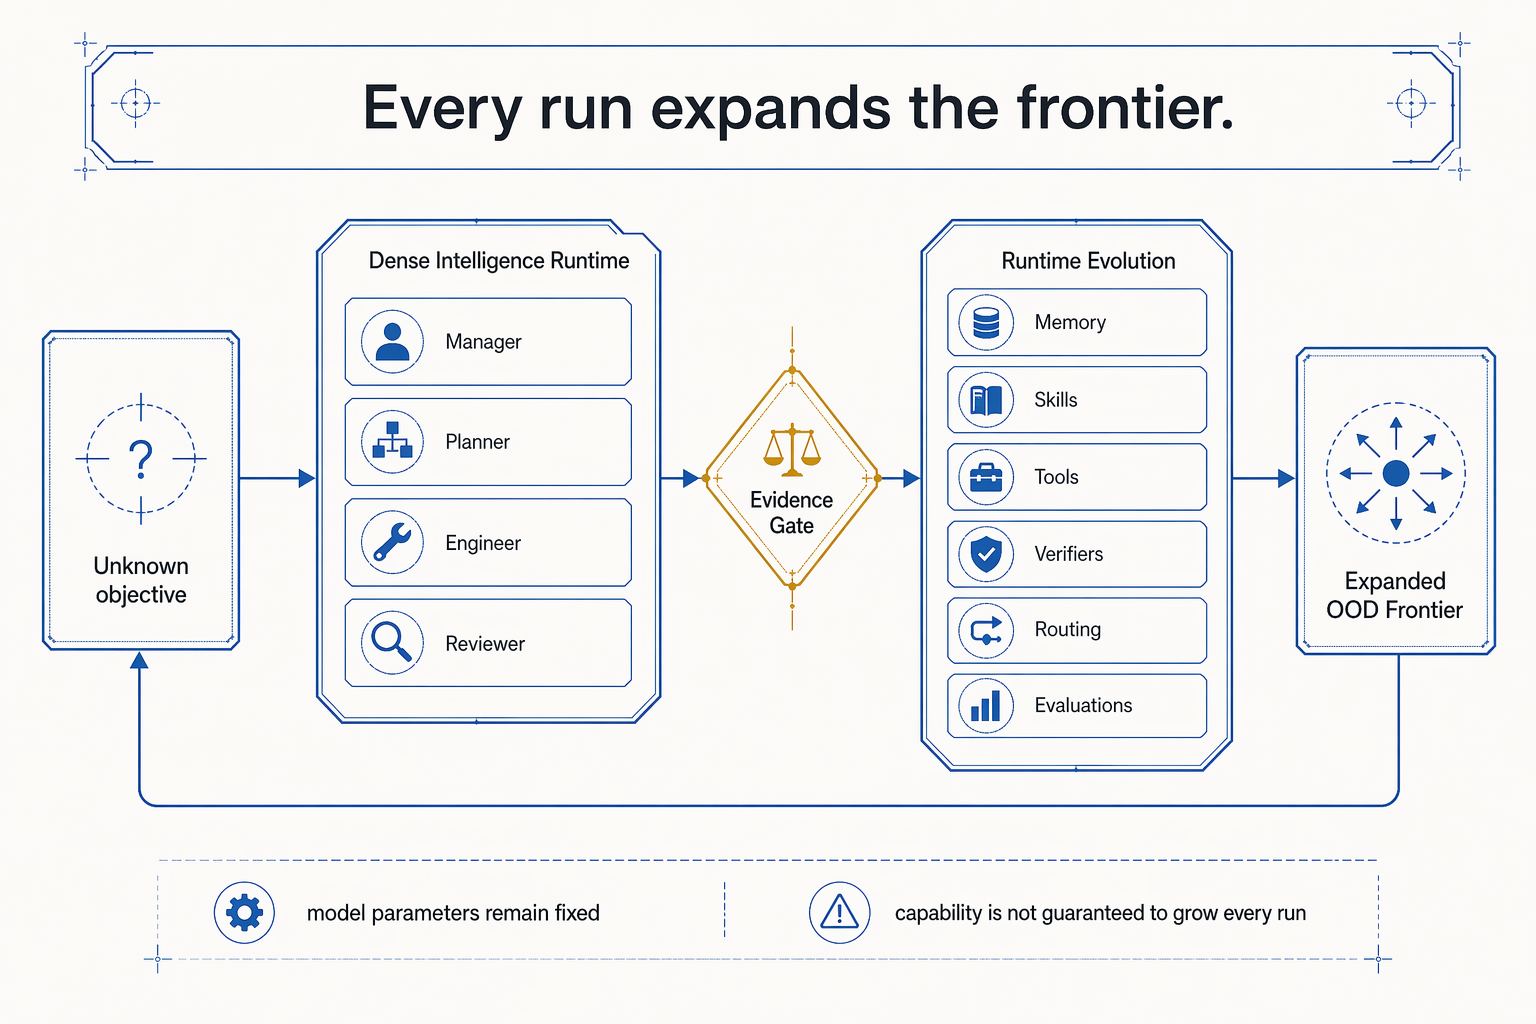
\includegraphics[width=0.88\textwidth]{figures/master_spine.png}
\caption{The expanding-frontier spine. An unknown, out-of-distribution objective
enters a dense-intelligence runtime driven by four persistent roles; verified work
passes an evidence gate; the gate updates durable runtime state; and the enlarged
runtime meets the next unknown task from a higher floor. Model parameters remain
fixed, and capability is not guaranteed to grow on every run.}
\label{fig:spine}
\end{figure}

\begin{table}[H]
\small
\renewcommand{\arraystretch}{1.25}
\begin{tabularx}{\linewidth}{@{}>{\raggedright\arraybackslash}X >{\raggedright\arraybackslash}X@{}}
\toprule
{\bfseries\color{deepblue}What this report claims} &
{\bfseries\color{graphitesoft}What it does not claim} \\
\midrule
Argus is engineered as a persistent, role-separated runtime that keeps decision,
execution, and verification coupled over long horizons. &
That the infrastructure is more capable than the model, or substitutes heuristics
for the agent's scientific judgment. \\
\addlinespace
Each run's reviewer-verified evidence updates durable runtime state --- memory,
skills, tools, verifiers, routing, evaluations --- with model parameters fixed. &
Monotone empirical capability growth: a run may fail, return only a negative
result, or add nothing verified. \\
\addlinespace
Six public arena results, each a scoped claim under its stated protocol, hardware,
and evidence tier. &
Universal state of the art, or superiority over all human researchers or other
systems. \\
\addlinespace
A 41-paper portfolio compared only to human-authored literature, reported as a
de-duplicated inventory. &
An accepted autonomous publication, or a count of accepted papers. \\
\addlinespace
Reliability and auditability by construction: bounded budgets, one completion
authority, an append-only evidence tape. &
Correctness, safety, or performance outside the exact protocols each result is
measured under. \\
\bottomrule
\end{tabularx}
\caption{The claim boundary the rest of the report is held to.}
\label{tab:claimboundary}
\end{table}

Argus publishes a live public record~\cite{argus_results}. This report reproduces
its six current arena results (Section~\ref{sec:results},
Figure~\ref{fig:results}), each with the protocol and hardware it was measured
under and its published reference: NVIDIA SOL-ExecBench (B200, 101 kernels; global
rank \#6 with two head-to-head wins over Recursive~\cite{recursive2026firststeps}),
nanochat on B200 (0.9636 BPB vs.\ human SOTA 0.9646) and H100 (0.9855 vs.\ 0.9879
BPB), the nanoGPT speedrun (79.77\,s vs.\ the same-device human record 80.18\,s,
$N{=}10$), AARRI-Bench (63/82, 76.8\% vs.\ the paper-reported best 68.3\%), and
Arbor's site-reported system comparison; two of the six --- the nanoGPT speedrun
and nanochat on B200 --- additionally carry committed artifact-digest records,
while the other four remain website snapshots, and that distinction is kept
visible throughout (Section~\ref{sec:evidence}). Separately, the public research
page~\cite{argus_research} lists a portfolio of \textbf{41 papers} --- 35
manuscripts and 6 drafts across six research programs
(Section~\ref{sec:portfolio}, Figure~\ref{fig:portfolio}) --- compared only to
human-authored literature and baselines, and reported as a de-duplicated inventory
rather than a count of accepted papers.

\begin{callout}[Design objective, not a measured guarantee]
``Every run leaves the system more capable'' is the design objective: a run may
fail, produce only a negative result, or add no verified capability. The report
does not claim monotone empirical capability growth.
\end{callout}
